%% approx.tex %%
  \subsection{Bref rappel des algorithmes}
  \begin{frame}
   \frametitle{Rappel}

   \begin{block}{Algorithme du projet (sommets non feuilles)}
    \begin{itemize}
     \item Calcul d'un arbre couvrant par parcours en profondeur
     \item Couverture = ensemble des sommets non feuilles (par parcours
	   en profondeur)
    \end{itemize}
   \end{block}

   \begin{block}{Algorithme du cours (couplage maximal)}
    \begin{itemize}
     \item Couverture = ensemble des sommets d'un couplage maximal
    \end{itemize}
   \end{block}

   \begin{block}{Complexités}
    \begin{itemize}
     \item Algorithme du projet : linéaire car consiste en deux parcours
	   en profondeur l'un après l'autre.
     \item Avec une structure de graphe adapté : linéaire.
    \end{itemize}
   \end{block}
  \end{frame}

  \subsection{Comparaison}
  \begin{frame}
   \frametitle{Comparaison des algorithmes d'approximation (1/3)}
   
   \begin{center}
    \begin{block}{Données : Graphe de comparaison \emph{Pise}}
     \begin{figure}[!ht]
      \begin{tikzpicture}[font=\small]
       \tikzstyle{level 1}=[level distance=0.8cm, sibling distance=0.8cm]
       \tikzstyle{childnode}=[rounded corners]
       \tikzstyle{marknode}=[fill=red!30, rounded corners]
       \tikzstyle{edge from parent}=[draw,thick]
       \node {0} 
        child {node[childnode] {1} 
         child {node[childnode] {2}
          child {node[childnode] {3}
          }
         }
         child {node[childnode] {4}
          child {node[childnode] {5}
          }
          child {node[childnode] {6} 
           child {node[childnode] {7}
           }
           child {node[childnode] {8}
            child {node[childnode] {9}
            }
            child {node[childnode] {10}
             child {node[childnode] {11}
             }
             child {node[childnode] {12}
              child {node[childnode] {13}
              }
             }
            }
           }
          }
         }
        };
      \end{tikzpicture}
     \end{figure}
    \end{block}
   \end{center}
  \end{frame}

  \begin{frame}
   \frametitle{Comparaison des algorithmes d'approximation (2/3)}

   \setlength{\tabcolsep}{1cm}
   \begin{center}
    \begin{block}{Comparaison des solutions sur le graphe \emph{Pise}}
     \begin{tabular}{cc}
      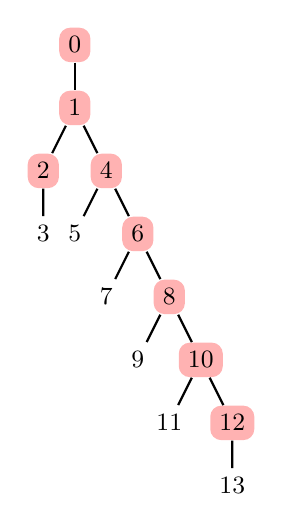
\begin{tikzpicture}[font=\small]
       \tikzstyle{level 1}=[level distance=0.8cm, sibling distance=0.8cm]
       \tikzstyle{childnode}=[rounded corners]
       \tikzstyle{marknode}=[fill=red!30, rounded corners]
       \tikzstyle{edge from parent}=[draw,thick]
       \node[childnode, fill=red!30] {0} 
        child {node[childnode,fill=red!30] {1} 
         child {node[childnode,fill=red!30] {2}
          child {node[childnode] {3}
          }
         }
         child {node[childnode,fill=red!30] {4}
          child {node[childnode] {5}
          }
          child {node[childnode,fill=red!30] {6} 
           child {node[childnode] {7}
           }
           child {node[childnode,fill=red!30] {8}
            child {node[childnode] {9}
            }
            child {node[childnode,fill=red!30] {10}
             child {node[childnode] {11}
             }
             child {node[childnode,fill=red!30] {12}
              child {node[childnode] {13}
              }
             }
            }
           }
          }
         }
        };
      \end{tikzpicture}
      &
      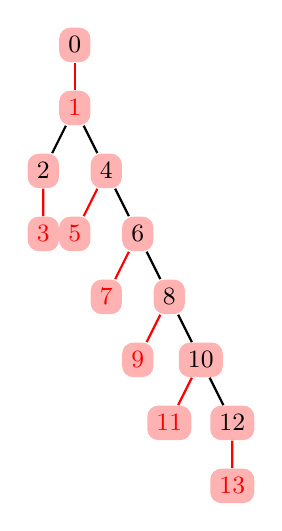
\begin{tikzpicture}[font=\small]
       \tikzstyle{level 1}=[level distance=0.8cm, sibling distance=0.8cm]
       \tikzstyle{childnode}=[rounded corners, fill=red!30]
       \tikzstyle{marknode}=[fill=red!30, rounded corners]
       \tikzstyle{edge from parent}=[draw,thick]
       \node[childnode] {0} 
        child[red] {node[childnode] {\Cb{1}} 
         child[black] {node[childnode] {\Cb{2}}
          child[red] {node[childnode] {\Cb{3}}
          }
         }
         child[black] {node[childnode] {\Cb{4}}
          child[red] {node[childnode] {\Cb{5}}
          }
          child[black] {node[childnode] {\Cb{6}}
           child[red] {node[childnode] {\Cb{7}}
           }
           child[black] {node[childnode] {\Cb{8}}
            child[red] {node[childnode] {\Cb{9}}
            }
            child[black] {node[childnode] {\Cb{10}}
             child[red] {node[childnode] {\Cb{11}}
             }
             child[black] {node[childnode] {\Cb{12}}
              child[red] {node[childnode] {\Cb{13}}
              }
             }
            }
           }
          }
         }
        };
      \end{tikzpicture}\\
      $C_{projet} = \{0,1,2,4,6,8,10,12\}$ & $C_{cours} = V$\\
     \end{tabular}
    \end{block}
   \end{center}
  \end{frame}

  \begin{frame}
   \frametitle{Comparaison des algorithmes d'approximation (3/3)}

   \begin{block}{Tableau de comparaison}
    \begin{figure}[!ht]
     \begin{center}
      \footnotesize
      \begin{tabular}{|c|c|c||c|c||c|c|}
       \cline{2-7}
       \multicolumn{1}{c|}{} & \multicolumn{2}{|c||}{jeuPise.gin}
       &\multicolumn{2}{|c||}{testTree100.gin} &
       \multicolumn{2}{|c|}{testTree1000.gin}\\ 
       \cline{2-7}
       \multicolumn{1}{c|}{} & algoP & algoC & algoP & algoC & algoP &
       algoC\\
       \hline
       Temps d'execution(en $\mu$s) & 58.5808 & 1.12014 & 400.344 &
       5.82175 & 3911.25 & 56.8837\\
       \hline
       Taille de la couverture & 8 & 14 & 38 & 58 & 365 & 576\\
       \hline
       \hline
       Taille couverture optimale & \multicolumn{2}{|c||}{7} &
		   \multicolumn{2}{|c||}{31} &
       \multicolumn{2}{|c|}{325}\\ 
       \hline
      \end{tabular}
      \caption{Tableau comparatif des exécutions des algorithmes sur
      plusieurs exemples.\label{tableau}} 
     \end{center}
    \end{figure}  
   \end{block}
  \end{frame}
